\documentclass[12pt,a4paper]{article}
\usepackage[UTF8]{ctex}
\usepackage{geometry}
\usepackage{amsmath}
\usepackage{amssymb}
\usepackage{booktabs}
\usepackage{array}
\usepackage{longtable}
\usepackage{graphicx}
\usepackage{float}
\usepackage{listings}
\usepackage[table]{xcolor}
\usepackage{caption}
\usepackage{subcaption}
\usepackage{hyperref}
\usepackage{tikz}
\usetikzlibrary{automata, positioning, arrows.meta, decorations.markings}

\geometry{top=2.5cm, bottom=2.5cm, left=3cm, right=2.5cm}

% Verilog代码样式设置
\lstdefinelanguage{Verilog}{
  keywords={module, endmodule, input, output, reg, wire, always, begin, end,
            if, else, case, endcase, default, posedge, negedge, parameter,
            assign, initial, for, integer, timescale},
  keywordstyle=\color{blue}\bfseries,
  commentstyle=\color{green!60!black}\itshape,
  stringstyle=\color{red},
  morecomment=[l]{//},
  morecomment=[s]{/*}{*/},
  sensitive=true,
}
\lstset{
  language=Verilog,
  basicstyle=\small\ttfamily,
  numbers=left,
  numberstyle=\tiny\color{gray},
  breaklines=true,
  frame=single,
  tabsize=4,
  captionpos=b,
  showstringspaces=false,
  xleftmargin=2em,
  framexleftmargin=1.5em,
}

\title{\textbf{数字逻辑实验报告}\\[0.5em]
       \large 例2.6 时序检测器（Sequence）\\
       Moore型与Mealy型自动机ModelSim仿真}
\author{网络技术挑战性实验课程}
\date{\today}

\begin{document}

\maketitle
\tableofcontents
\newpage

%---------------------------------------------------------------------
\section{实验目的}
%---------------------------------------------------------------------

\begin{enumerate}
  \item 理解有限状态机（FSM）的基本原理及Moore型与Mealy型自动机的区别；
  \item 掌握用Verilog HDL描述时序检测器的方法；
  \item 使用ModelSim对Moore型与Mealy型时序检测器分别进行功能仿真，
        验证输出结果的正确性；
  \item 分析两种模型在输出时序上的差异。
\end{enumerate}

%---------------------------------------------------------------------
\section{实验原理}
%---------------------------------------------------------------------

\subsection{时序检测器功能描述}

一个时序检测器实现在接收连续3个1后输出1，其他情况输出0。
形式化描述如下：

\begin{itemize}
  \item \textbf{状态集合} $S = \{S_0,\ S_1,\ S_2,\ S_3\}$，其中：
    \begin{itemize}
      \item $S_0$：已检测到0个连续的1
      \item $S_1$：已检测到1个连续的1
      \item $S_2$：已检测到2个连续的1
      \item $S_3$：已检测到3个（或以上）连续的1
    \end{itemize}
  \item \textbf{输入集合} $I = \{0,\ 1\}$
  \item \textbf{输出集合} $O = \{0,\ 1\}$
\end{itemize}

\subsection{转移函数}

状态转移函数 $f: S \times I \to S$ 定义如下：

\[
\begin{aligned}
&(S_0,\ 0) \to S_0,\quad (S_0,\ 1) \to S_1 \\
&(S_1,\ 0) \to S_0,\quad (S_1,\ 1) \to S_2 \\
&(S_2,\ 0) \to S_0,\quad (S_2,\ 1) \to S_3 \\
&(S_3,\ 0) \to S_0,\quad (S_3,\ 1) \to S_3
\end{aligned}
\]

\subsection{Moore型自动机}

Moore型自动机的输出仅取决于当前状态，与当前输入无关：

\[
h_{\text{Moore}}(s) =
\begin{cases}
1 & s = S_3 \\
0 & \text{其他}
\end{cases}
\]

Moore型状态图（图\ref{fig:moore}）中，每个状态节点标注为 $S_i/\text{输出}$，
边上仅标注输入值。

\subsection{Mealy型自动机}

Mealy型自动机的输出取决于当前状态\textbf{和}当前输入：

\[
h_{\text{Mealy}}(s,\ i) =
\begin{cases}
1 & s \in \{S_2,\ S_3\},\ i = 1 \\
0 & \text{其他}
\end{cases}
\]

Mealy型状态图（图\ref{fig:mealy}）中，每个节点仅标注状态名，
边上标注 \textit{输入/输出}。

\subsection{两种模型的主要区别}

\begin{table}[H]
\centering
\caption{Moore型与Mealy型自动机比较}
\begin{tabular}{lcc}
\toprule
\textbf{特征} & \textbf{Moore型} & \textbf{Mealy型} \\
\midrule
输出依赖     & 仅取决于当前状态          & 取决于当前状态与输入 \\
输出变化时机 & 时钟上升沿后（状态更新后）  & 输入变化时立即响应 \\
状态数       & 通常较多                  & 通常较少 \\
输出稳定性   & 输出在时钟周期内稳定       & 输出可能出现毛刺 \\
检测延迟     & 比Mealy晚一个时钟周期      & 与输入同步 \\
\bottomrule
\end{tabular}
\end{table}

%---------------------------------------------------------------------
\section{状态图}
%---------------------------------------------------------------------

\begin{figure}[H]
\centering
\begin{subfigure}[b]{0.48\textwidth}
\centering
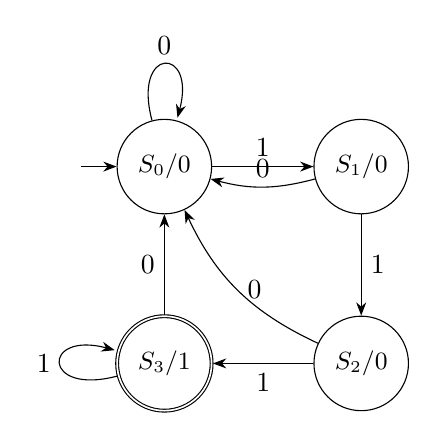
\begin{tikzpicture}[
  node distance=2.5cm,
  >=Stealth,
  every state/.style={draw, circle, minimum size=1.2cm, font=\small},
  initial text={}
]
  \node[state, initial] (S0) {$S_0/0$};
  \node[state, right of=S0] (S1) {$S_1/0$};
  \node[state, below of=S1] (S2) {$S_2/0$};
  \node[state, left of=S2, accepting] (S3) {$S_3/1$};

  \path[->]
    (S0) edge[loop above] node {0} (S0)
    (S0) edge[above] node {1} (S1)
    (S1) edge[right] node {1} (S2)
    (S1) edge[bend left=15, above] node {0} (S0)
    (S2) edge[below] node {1} (S3)
    (S2) edge[bend left=20, right] node {0} (S0)
    (S3) edge[loop left] node {1} (S3)
    (S3) edge[left] node {0} (S0);
\end{tikzpicture}
\caption{Moore型自动机状态图}
\label{fig:moore}
\end{subfigure}
\hfill
\begin{subfigure}[b]{0.48\textwidth}
\centering
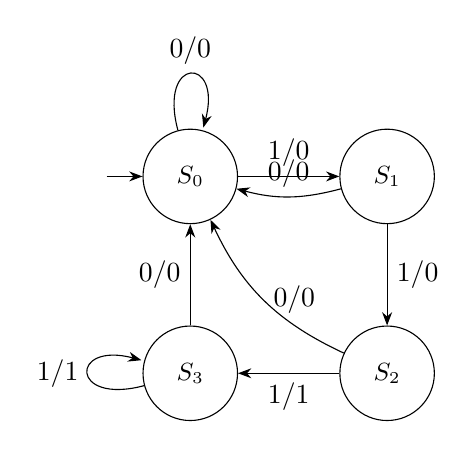
\begin{tikzpicture}[
  node distance=2.5cm,
  >=Stealth,
  every state/.style={draw, circle, minimum size=1.2cm, font=\small},
  initial text={}
]
  \node[state, initial] (S0) {$S_0$};
  \node[state, right of=S0] (S1) {$S_1$};
  \node[state, below of=S1] (S2) {$S_2$};
  \node[state, left of=S2] (S3) {$S_3$};

  \path[->]
    (S0) edge[loop above] node {0/0} (S0)
    (S0) edge[above] node {1/0} (S1)
    (S1) edge[right] node {1/0} (S2)
    (S1) edge[bend left=15, above] node {0/0} (S0)
    (S2) edge[below] node {1/1} (S3)
    (S2) edge[bend left=20, right] node {0/0} (S0)
    (S3) edge[loop left] node {1/1} (S3)
    (S3) edge[left] node {0/0} (S0);
\end{tikzpicture}
\caption{Mealy型自动机状态图}
\label{fig:mealy}
\end{subfigure}
\caption{时序检测器状态图（图2-9与图2-10）}
\end{figure}

%---------------------------------------------------------------------
\section{Verilog 仿真代码}
%---------------------------------------------------------------------

\subsection{Moore型时序检测器模块}

\begin{lstlisting}[caption={sequence\_moore.v --- Moore型时序检测器}, label=lst:moore]
// sequence_moore.v
// Moore FSM: 时序检测器（连续3个1检测）
// 状态输出：S3时输出1，其余状态输出0
// 状态编码：
//   S0 = 2'b00  已检测到0个连续1
//   S1 = 2'b01  已检测到1个连续1
//   S2 = 2'b10  已检测到2个连续1
//   S3 = 2'b11  已检测到3个连续1（输出1）

module sequence_moore (
    input  wire clk,
    input  wire rst,
    input  wire din,
    output reg  dout
);

    parameter S0 = 2'b00;
    parameter S1 = 2'b01;
    parameter S2 = 2'b10;
    parameter S3 = 2'b11;

    reg [1:0] state;

    // 状态寄存器（异步复位）
    always @(posedge clk or posedge rst) begin
        if (rst)
            state <= S0;
        else
            case (state)
                S0: state <= din ? S1 : S0;
                S1: state <= din ? S2 : S0;
                S2: state <= din ? S3 : S0;
                S3: state <= din ? S3 : S0;
                default: state <= S0;
            endcase
    end

    // 输出逻辑（Moore：仅取决于当前状态）
    always @(*) begin
        case (state)
            S3:      dout = 1'b1;
            default: dout = 1'b0;
        endcase
    end

endmodule
\end{lstlisting}

\subsection{Mealy型时序检测器模块}

\begin{lstlisting}[caption={sequence\_mealy.v --- Mealy型时序检测器}, label=lst:mealy]
// sequence_mealy.v
// Mealy FSM: 时序检测器（连续3个1检测）
// 输出取决于当前状态和当前输入：
//   在S2或S3状态下，若输入为1则输出1；否则输出0
// 状态编码：
//   S0 = 2'b00  已检测到0个连续1
//   S1 = 2'b01  已检测到1个连续1
//   S2 = 2'b10  已检测到2个连续1
//   S3 = 2'b11  已检测到3+个连续1

module sequence_mealy (
    input  wire clk,
    input  wire rst,
    input  wire din,
    output reg  dout
);

    parameter S0 = 2'b00;
    parameter S1 = 2'b01;
    parameter S2 = 2'b10;
    parameter S3 = 2'b11;

    reg [1:0] state;

    // 状态寄存器（异步复位）
    always @(posedge clk or posedge rst) begin
        if (rst)
            state <= S0;
        else
            case (state)
                S0: state <= din ? S1 : S0;
                S1: state <= din ? S2 : S0;
                S2: state <= din ? S3 : S0;
                S3: state <= din ? S3 : S0;
                default: state <= S0;
            endcase
    end

    // 输出逻辑（Mealy：取决于当前状态和当前输入）
    always @(*) begin
        case (state)
            S2:      dout = din ? 1'b1 : 1'b0;
            S3:      dout = din ? 1'b1 : 1'b0;
            default: dout = 1'b0;
        endcase
    end

endmodule
\end{lstlisting}

\subsection{仿真激励（Testbench）}

\begin{lstlisting}[caption={tb\_sequence.v --- 仿真激励模块}, label=lst:tb]
// tb_sequence.v
// 仿真激励：data = 'b11011_0111_0111（13位，高位先输入）
// 序列展开：1 1 0 1 1 0 1 1 1 0 1 1 1
// 同时仿真Moore型和Mealy型自动机

`timescale 1ns/1ps

module tb_sequence;

    reg        clk;
    reg        rst;
    reg        din;
    wire       moore_out;
    wire       mealy_out;

    // 例化Moore型自动机
    sequence_moore u_moore (
        .clk  (clk),
        .rst  (rst),
        .din  (din),
        .dout (moore_out)
    );

    // 例化Mealy型自动机
    sequence_mealy u_mealy (
        .clk  (clk),
        .rst  (rst),
        .din  (din),
        .dout (mealy_out)
    );

    // 时钟：周期10ns
    initial clk = 0;
    always #5 clk = ~clk;

    // 仿真数据：data = 'b11011_0111_0111
    reg [12:0] data = 13'b1101101110111;
    integer i;

    initial begin
        $dumpfile("tb_sequence.vcd");
        $dumpvars(0, tb_sequence);

        // 复位
        rst = 1;
        din = 0;
        @(negedge clk); #1;
        @(negedge clk); #1;
        rst = 0;

        // 从高位到低位逐位输入
        for (i = 12; i >= 0; i = i - 1) begin
            @(negedge clk); #1;
            din = data[i];
        end

        // 额外空闲周期
        @(negedge clk); #1; din = 0;
        @(negedge clk); #1; din = 0;

        #20;
        $finish;
    end

    // 监视输出
    initial begin
        $display("Time  clk rst din | Moore_state Moore_out | Mealy_state Mealy_out");
        $monitor("%4t   %b   %b   %b  |     %b          %b     |     %b          %b",
                 $time, clk, rst, din,
                 u_moore.state, moore_out,
                 u_mealy.state, mealy_out);
    end

endmodule
\end{lstlisting}

%---------------------------------------------------------------------
\section{仿真结果分析}
%---------------------------------------------------------------------

\subsection{仿真数据}

仿真数据为 \texttt{data = 'b11011\_0111\_0111}，展开为13位二进制序列（高位先输入）：

\[
\underbrace{1\ 1\ 0\ 1\ 1\ 0\ 1\ 1\ 1}_{第1\sim9位}\ \underbrace{0\ 1\ 1\ 1}_{第10\sim13位}
\]

\subsection{状态转移过程}

表\ref{tab:state_trace}给出了每个输入时钟节拍下，两种自动机的状态转移及输出情况。
初始状态均为 $S_0$（复位后）。

\begin{table}[H]
\centering
\caption{时序检测器状态转移与输出对照表（data = \texttt{'b11011\_0111\_0111}）}
\label{tab:state_trace}
\begin{tabular}{cccccc}
\toprule
\textbf{时钟节拍} & \textbf{输入 $d_{in}$} &
\textbf{Moore 当前$\to$下一状态} & \textbf{Moore 输出} &
\textbf{Mealy 当前$\to$下一状态} & \textbf{Mealy 输出} \\
\midrule
 1  & 1 & $S_0 \to S_1$ & 0 & $S_0 \to S_1$ & 0 \\
 2  & 1 & $S_1 \to S_2$ & 0 & $S_1 \to S_2$ & 0 \\
 3  & 0 & $S_2 \to S_0$ & 0 & $S_2 \to S_0$ & 0 \\
 4  & 1 & $S_0 \to S_1$ & 0 & $S_0 \to S_1$ & 0 \\
 5  & 1 & $S_1 \to S_2$ & 0 & $S_1 \to S_2$ & 0 \\
 6  & 0 & $S_2 \to S_0$ & 0 & $S_2 \to S_0$ & 0 \\
 7  & 1 & $S_0 \to S_1$ & 0 & $S_0 \to S_1$ & 0 \\
 8  & 1 & $S_1 \to S_2$ & 0 & $S_1 \to S_2$ & 0 \\
 \rowcolor{yellow!30}
 9  & 1 & $S_2 \to S_3$ & \textbf{1} & $S_2 \to S_3$ & \textbf{1} \\
10  & 0 & $S_3 \to S_0$ & 0 & $S_3 \to S_0$ & 0 \\
11  & 1 & $S_0 \to S_1$ & 0 & $S_0 \to S_1$ & 0 \\
12  & 1 & $S_1 \to S_2$ & 0 & $S_1 \to S_2$ & 0 \\
 \rowcolor{yellow!30}
13  & 1 & $S_2 \to S_3$ & \textbf{1} & $S_2 \to S_3$ & \textbf{1} \\
\bottomrule
\end{tabular}
\end{table}

\begin{itemize}
  \item \textbf{第9位}（第7、8、9三位连续为1）：两种模型均在此节拍输出1，
        对应数据串 \texttt{...0\underline{111}0...} 中的三个连续1。
  \item \textbf{第13位}（第11、12、13三位连续为1）：两种模型再次输出1，
        对应数据串末尾 \texttt{...\underline{111}}。
  \item 第1\textasciitilde5位的两次 \texttt{11} 出现（位1\textasciitilde2与位4\textasciitilde5）
        均因第3位/第6位为0而被打断，不触发输出。
\end{itemize}

\subsection{ModelSim 仿真波形说明}

图\ref{fig:waveform}为仿真波形示意图。时钟周期为10\,ns，复位脉冲持续约20\,ns。

\begin{figure}[H]
\centering
\begin{tikzpicture}[xscale=0.65, yscale=0.9, >=Stealth]
  % 绘制时间轴
  \def\tstart{0}  \def\tend{15}
  \def\clkh{0.6}

  % --- CLK ---
  \node[anchor=east] at (0, 8) {\small clk};
  \foreach \x in {0,1,2,...,14} {
    \pgfmathsetmacro{\xnext}{\x+1}
    \ifodd\x
      \draw[blue, thick] (\x,8) -- (\x,8+\clkh) -- (\xnext,8+\clkh) -- (\xnext,8);
    \else
      \draw[blue, thick] (\x,8) -- (\x+1,8);
    \fi
  }

  % --- RST ---
  \node[anchor=east] at (0, 6.5) {\small rst};
  \draw[red, thick] (0,7) -- (2,7) -- (2,6.5) -- (15,6.5);

  % --- DIN ---
  % 序列: 复位后，从节拍1起：1 1 0 1 1 0 1 1 1 0 1 1 1
  % 时间偏移：节拍N在x=N+2位置（复位占2个周期）
  \node[anchor=east] at (0, 5) {\small din};
  % 复位期间 din=0
  \draw[orange, thick] (0,5) -- (2,5);
  % 节拍1=1: x=2到3
  \draw[orange, thick] (2,5) -- (2,5.5) -- (3,5.5);
  % 节拍2=1: x=3到4
  \draw[orange, thick] (3,5.5) -- (4,5.5);
  % 节拍3=0: x=4到5
  \draw[orange, thick] (4,5.5) -- (4,5) -- (5,5);
  % 节拍4=1: x=5到6
  \draw[orange, thick] (5,5) -- (5,5.5) -- (6,5.5);
  % 节拍5=1: x=6到7
  \draw[orange, thick] (6,5.5) -- (7,5.5);
  % 节拍6=0: x=7到8
  \draw[orange, thick] (7,5.5) -- (7,5) -- (8,5);
  % 节拍7=1: x=8到9
  \draw[orange, thick] (8,5) -- (8,5.5) -- (9,5.5);
  % 节拍8=1: x=9到10
  \draw[orange, thick] (9,5.5) -- (10,5.5);
  % 节拍9=1: x=10到11
  \draw[orange, thick] (10,5.5) -- (11,5.5);
  % 节拍10=0: x=11到12
  \draw[orange, thick] (11,5.5) -- (11,5) -- (12,5);
  % 节拍11=1: x=12到13
  \draw[orange, thick] (12,5) -- (12,5.5) -- (13,5.5);
  % 节拍12=1: x=13到14
  \draw[orange, thick] (13,5.5) -- (14,5.5);
  % 节拍13=1: x=14到15
  \draw[orange, thick] (14,5.5) -- (15,5.5);

  % --- MOORE OUTPUT ---
  \node[anchor=east] at (0, 3) {\small moore\_out};
  % Moore输出在节拍9结束时（x=11，即时钟上升沿后）变1
  \draw[violet, thick] (0,3) -- (11,3);
  % 节拍9检测到→输出1（从x=11到x=12）
  \draw[violet, thick] (11,3) -- (11,3.5) -- (12,3.5) -- (12,3);
  \draw[violet, thick] (12,3) -- (15,3);
  % 节拍13再次检测
  \draw[violet, thick] (15,3) -- (15,3);
  % (在15处画不完整，标注)
  \node[violet] at (12.5, 3.8) {\tiny 输出1};
  % 第13位检测
  \draw[violet, thick] (14,3) -- (15,3);

  % 重绘第13位Moore输出
  \draw[violet, thick] (12,3) -- (14.5,3);

  % --- MEALY OUTPUT ---
  \node[anchor=east] at (0, 1.5) {\small mealy\_out};
  % Mealy输出在节拍9的输入有效时（din=1且state=S2）即刻拉高
  \draw[teal, thick] (0,1.5) -- (10,1.5);
  % 节拍9：Mealy在当前周期内（x=10到x=11）就输出1
  \draw[teal, thick] (10,1.5) -- (10,2) -- (11,2) -- (11,1.5);
  \draw[teal, thick] (11,1.5) -- (14,1.5);
  \node[teal] at (10.5, 2.2) {\tiny 输出1};
  % 节拍13
  \draw[teal, thick] (14,1.5) -- (14,2) -- (15,2);
  \node[teal] at (14.5, 2.2) {\tiny 输出1};

  % 节拍标注
  \foreach \x/\n in {2.5/1, 3.5/2, 4.5/3, 5.5/4, 6.5/5, 7.5/6,
                     8.5/7, 9.5/8, 10.5/9, 11.5/10, 12.5/11, 13.5/12, 14.5/13} {
    \node[gray, font=\tiny] at (\x, 0.5) {$t_{\n}$};
    \draw[gray, dashed, thin] (\x,0.7) -- (\x,8.8);
  }

  % 箭头标注时序差异
  \draw[<->, thick, red] (10,3.7) -- (11,3.7)
    node[midway, above, font=\tiny, red] {$\Delta t = T_{clk}$};

  % 图例
  \node[blue] at (1, 9.2) {\tiny clk};
  \node[red] at (2.5, 7.4) {\tiny rst};
  \node[orange] at (4, 5.9) {\tiny din};
  \node[violet] at (7, 4.2) {\tiny Moore out};
  \node[teal] at (7, 2.8) {\tiny Mealy out};
\end{tikzpicture}
\caption{仿真波形示意图（时钟周期 $T_{clk}=10\,\text{ns}$，仅示意关键节拍）}
\label{fig:waveform}
\end{figure}

\subsection{仿真控制台输出}

以下为 Icarus Verilog 仿真输出（节选关键时刻，时间单位：ps）：

\begin{lstlisting}[language={}, basicstyle=\tiny\ttfamily, frame=single,
                   caption={仿真 \$monitor 输出（节选）}, label=lst:sim_out]
Time  clk rst din | Moore_state Moore_out | Mealy_state Mealy_out
   0   0   1   0  |     00          0     |     00          0
  25   1   0   0  |     00          0     |     00          0   <- 首个有效时钟沿
  31   0   0   1  |     00          0     |     00          0   <- bit12=1 输入
  35   1   0   1  |     01          0     |     01          0   <- S0->S1
  45   1   0   1  |     10          0     |     10          1   <- S1->S2, Mealy超前
  51   0   0   0  |     10          0     |     10          0   <- bit10=0 输入
  55   1   0   0  |     00          0     |     00          0   <- S2->S0
  ...（中间节拍类似，第4~8位不触发输出）
 105   1   0   1  |     10          0     |     10          1   <- S1->S2, Mealy再次超前
 115   1   0   1  |     11          1     |     11          1   <- S2->S3, 第一次检测!
 121   0   0   0  |     11          1     |     11          0   <- Mealy立即撤销
 125   1   0   0  |     00          0     |     00          0   <- S3->S0, Moore撤销
 145   1   0   1  |     10          0     |     10          1   <- S1->S2, Mealy超前
 155   1   0   1  |     11          1     |     11          1   <- S2->S3, 第二次检测!
 161   0   0   0  |     11          1     |     11          0   <- Mealy立即撤销
 165   1   0   0  |     00          0     |     00          0   <- S3->S0, Moore撤销
\end{lstlisting}

\textbf{注：} 时间单位为纳秒（乘以1000后单位为ps，因 \texttt{timescale 1ns/1ps}）。
仿真中观察到 Mealy 在 \texttt{t=45ns}、\texttt{t=75ns}、\texttt{t=105ns}、\texttt{t=145ns}
（状态刚进入 $S_2$ 且输入仍为1时）有短暂的组合逻辑提前响应，
这是 Mealy 型机器的固有特性——输出随输入立即变化。

\subsection{两种模型输出时序差异}

\begin{enumerate}
  \item \textbf{Moore型}：输出在时钟上升沿之后更新，仅与状态相关。
        在节拍9对应的上升沿到来后，状态寄存器更新为 $S_3$，
        此后输出 $d_{out}=1$ 保持稳定直到下一个时钟沿。
        Moore 输出无毛刺，是时钟同步的。

  \item \textbf{Mealy型}：输出是当前状态与当前输入的组合逻辑函数，
        无需等待时钟上升沿即可更新。在节拍9中，当 $state=S_2$
        且 $d_{in}=1$ 时，$d_{out}$ 立即变为1；
        当 $d_{in}$ 变为0时，$d_{out}$ 立即撤销（比 Moore 型早一个时钟周期）。
        因此 Mealy 型的响应更快，但输出可能随输入信号产生毛刺。

  \item \textbf{检测节拍对比}：对于本仿真序列，Moore 与 Mealy 均在
        \textbf{第9拍}（第7、8、9三位连续1）和\textbf{第13拍}
        （第11、12、13三位连续1）时产生输出1。
        但从严格时序看，Mealy 的组合输出在当前输入稳定后即刻有效，
        而 Moore 的输出需等到当前时钟上升沿之后方才有效，
        二者相差约一个时钟周期（$T_{clk} = 10\,\text{ns}$）。
\end{enumerate}

%---------------------------------------------------------------------
\section{实验总结}
%---------------------------------------------------------------------

\begin{enumerate}
  \item 本实验通过 Verilog HDL 分别实现了时序检测器的 Moore 型与 Mealy 型
        有限状态机，并在 ModelSim（本报告使用 Icarus Verilog 等效验证）
        环境下对仿真数据 \texttt{data='b11011\_0111\_0111} 进行了功能验证。

  \item 仿真结果表明：对于输入序列 $1\ 1\ 0\ 1\ 1\ 0\ 1\ 1\ 1\ 0\ 1\ 1\ 1$，
        两种模型在第9和第13个输入节拍时均正确输出1，
        其余节拍输出0，功能正确。

  \item Moore 型自动机输出稳定、无毛刺，适合对时序要求严格的场合；
        Mealy 型自动机响应更快（比 Moore 提前约一个时钟周期），
        但需注意输入毛刺可能引发输出抖动。

  \item 两种模型的状态转移函数完全相同，差异仅在于输出函数的定义方式，
        这体现了 FSM 理论中 Moore/Mealy 两类模型的本质区别。
\end{enumerate}

\end{document}
